

%%% This LaTeX source document can be used as the basis for your technical
%%% report. Intentionally stripped and simplified
%%% and commands should be adjusted for your particular paper - title, 
%%% author, citations, equations, etc.
% % Citations/references are in report.bib 

\documentclass[conference,backref=page]{acmsiggraph}
\usepackage{dblfloatfix}
\usepackage{graphicx}


\TOGonlineid{45678}
\TOGvolume{0}
\TOGnumber{0}
\TOGarticleDOI{1111111.2222222}
\TOGprojectURL{}
\TOGvideoURL{}
\TOGdataURL{}
\TOGcodeURL{}

% Include this so that citations show up in blue and the page information is included in the reference section
\hypersetup{
    colorlinks = true, 
    linkcolor = blue,
    anchorcolor = red,
    citecolor = blue, 
    filecolor = red, 
}


\title{Solving The Travelling Salesman Problem\\
	   A Report Analysing the Algorithms Used}

\author{Beej Persson\thanks{e-mail:40183743@live.napier.ac.uk} \\
Edinburgh Napier University\\
Algorithms and Data Structures (SET09117)}
\pdfauthor{Beej Persson}

\keywords{algorithms, data structures, travelling salesman, efficacy, efficiency, problem solving.}

\begin{document}

\maketitle

\raggedbottom

\begin{abstract}

The Travelling Salesman Problem is a common algorithmic problem often discussed in computer science. The problem itself is to find the shortest route of travel between all the desired cities without going to a city twice. This report looks to analyse two algorithmic solutions to this problem and compare them against each other. The first solution is the Nearest Neighbour algorithm whilst the second is a modified and enhanced version of that algorithm. Multiple tests were run to evaluate their efficacy, including measuring run time, comparing route lengths and increasing the number of cities.

\end{abstract}

\keywordlist

\section{Introduction}


\paragraph{The Problem}
Given a list of cities and their locations (and therefore the distances between each city), what is the shortest route from a starting city that travels to each city only once before returning to the starting city? Solving this problem is often not only about achieving the shortest possible route, there is a focus on optimisation: finding this shortest route in a reasonable time given the number of cities.

\paragraph{First Solution: Nearest Neighbour Basic}
The Nearest Neighbour algorithm used here solves the problem by starting with the first city in the file, checking the distances between it and all the other cities, picking the shortest distance then doing the same for that closest city with all the rest, whilst removing each previous city. This algorithm tends to return fairly short routes (although rarely the shortest) whilst also being fairly efficient. When used on a larger number of cities, the run time will still be comparatively low. This is due to it having an order of complexity of $n^2$, or $O(n^2)$, where the run time will increase in proportion to the problem size squared (for example the theoretical run time on a set of 10 cities will be 4 times bigger than on a set of 5, as $(10/5)^2 = 4$).

\paragraph{Second Solution: Nearest Neighbour Enhanced}
The Nearest Neighbour Enhanced algorithm uses a fairly simple adaptation to the previous algorithm. Instead of starting with the first city in the file, it will start with a random city and find the closest city to it and carry on from there. After that it will calculate the length of that route. It will do these two steps a number of times (specifically a tenth of the number of cities in the file) and then look over the list of lengths and pick the lowest route length found. This algorithm should consistently find lower route lengths at the expense of increased run time. As it is running the previous algorithm $n/10$ times (where n is the number of cities), its order of complexity is $O(n^3)$. This means that as the problem size increases, the run time will increase significantly (for example, the theoretical run time on a set of 10 cities will be 8 times bigger than on a set of 5, as $(10/5)^3 = 8$).


\section{Experimental Method}

\paragraph{Overview}
The algorithms were tested against each other and on a variety of problem instances, with differing numbers of cities in each problem instance. The time it took the algorithm to return a sorted list of cities from the original unsorted list was used as the Run Time. The Route Length results were determined by calculating the length of the route between all the cities in the order of the sorted cities list. Tests were repeated for each algorithm for every problem instance. The results used were the averages of these repeated tests.

\paragraph{Detailed description}
\begin{itemize}
\item {\bf Functionality of One Test}: Problem instance files containing a list of a certain number, $n$, of cities were loaded into an array list in Java. The algorithms sort this array list into an ordered list of cities, the order being the shortest route it found. The Run Time is calculated by finding the difference between the current time in milliseconds immediately before the algorithm is run and immediately after it returns a sorted list. This sorted list is then passed through a method that calculates the Route Length of the sorted cities in order. The Run Time and Route Length results were recorded for each test.
\item {\bf Testing Methodology}: For each of the chosen problem instances ten tests were run on each algorithm. For each test the results for the Run Time and the Route Length were then recorded in a table in an Excel file (see figure \ref{avgresultstable}). The average Run Time and Route Length for each algorithm were stored in a separate table ref:fig3 against the number of cities, $n$. This was the testing method used to produce the results and graphs analysed in this report.
\end{itemize}

\paragraph{Accuracy, Reliability and Reasoning for Testing Methodology}
 The number of cities in the file is initially known and is part of the file name. The number of cities in the array list (that the cities from the file are loaded into) is checked to match the number of cities in the file, and checked again after the algorithm is run. This is to ensure that the Route Length for the shortest route found is including every city in the problem instance and eliminate any artificially short routes. Nine problem instances were used, with an appropriately varying number of cities in each (ranging from 52 cities, up to 5915 cities) to help visualise the effect of $n$ on the Run Time of the two algorithms. Each test was run on the same PC, from the same code, with each result being recorded one at a time to reduce memory build up slowing down Run Time and improve the accuracy and repeatability of the results. Ten tests were run for each problem instance and for each algorithm and the average Run Times and Route Lengths were used for displaying the results to further improve reliability of the accuracy of the testing methodology.


\section{Results}
In this section of the {\bf Design document}, you should describe the tests that you are considering carrying out to test your evaluation and ensure that it works within its specified boundaries. In your {\bf Final report}, you will present the actual evaluation that you have carried out and reflect on its outcome. In particular, you may consider the actual performance of your simulation in relation to your initial goals. A comparison to relevant work would also be beneficial.

\begin{figure}[h]
	\begin{center}
		\resizebox{\columnwidth}{!}{%
		\begin{tabular}{lllll}
			& \multicolumn{4}{c}{Averages} \\ \cline{2-5} 
			\multicolumn{1}{l|}{} & \multicolumn{2}{c|}{\begin{tabular}[c]{@{}c@{}}Nearest\\   Neighbour Basic\end{tabular}} & \multicolumn{2}{c|}{\begin{tabular}[c]{@{}c@{}}Nearest\\   Neighbour Enhanced\end{tabular}} \\ \hline
			\multicolumn{1}{l|}{n} & \multicolumn{1}{l|}{Time / ms} & \multicolumn{1}{l|}{Route Length / units} & \multicolumn{1}{l|}{Time / ms} & Route Length / units \\ \hline
			\multicolumn{1}{l|}{52} & 0.6 & \multicolumn{1}{l|}{8,980.918} & 1.0 & 8,883.095 \\
			\multicolumn{1}{l|}{101} & 1.0 & \multicolumn{1}{l|}{825.242} & 2.5 & 759.497 \\
			\multicolumn{1}{l|}{159} & 1.6 & \multicolumn{1}{l|}{54,669.026} & 5.6 & 50,251.966 \\
			\multicolumn{1}{l|}{262} & 5.8 & \multicolumn{1}{l|}{3,241.467} & 19.9 & 2,920.326 \\
			\multicolumn{1}{l|}{493} & 4.9 & \multicolumn{1}{l|}{43,646.374} & 125.0 & 41,982.407 \\
			\multicolumn{1}{l|}{1060} & 13.3 & \multicolumn{1}{l|}{296,543.889} & 1,102.4 & 281,530.521 \\
			\multicolumn{1}{l|}{2103} & 44.2 & \multicolumn{1}{l|}{90,517.890} & 8,113.1 & 87,664.568 \\
			\multicolumn{1}{l|}{3795} & 137.1 & \multicolumn{1}{l|}{35,362.51} & 45,949.0 & 34,226.09 \\
			\multicolumn{1}{l|}{5915} & 336.4 & \multicolumn{1}{l|}{707,498.63} & 179,763.5 & 672,798.03
		\end{tabular}%
		}
	\end{center}
	\caption{A graph showing the Nearest Neighbour Basic algorithm's average run time compared against the number of cities in each problem instance.}
	\label{avgresultstable}
\end{figure}

\begin{figure*}[t]
	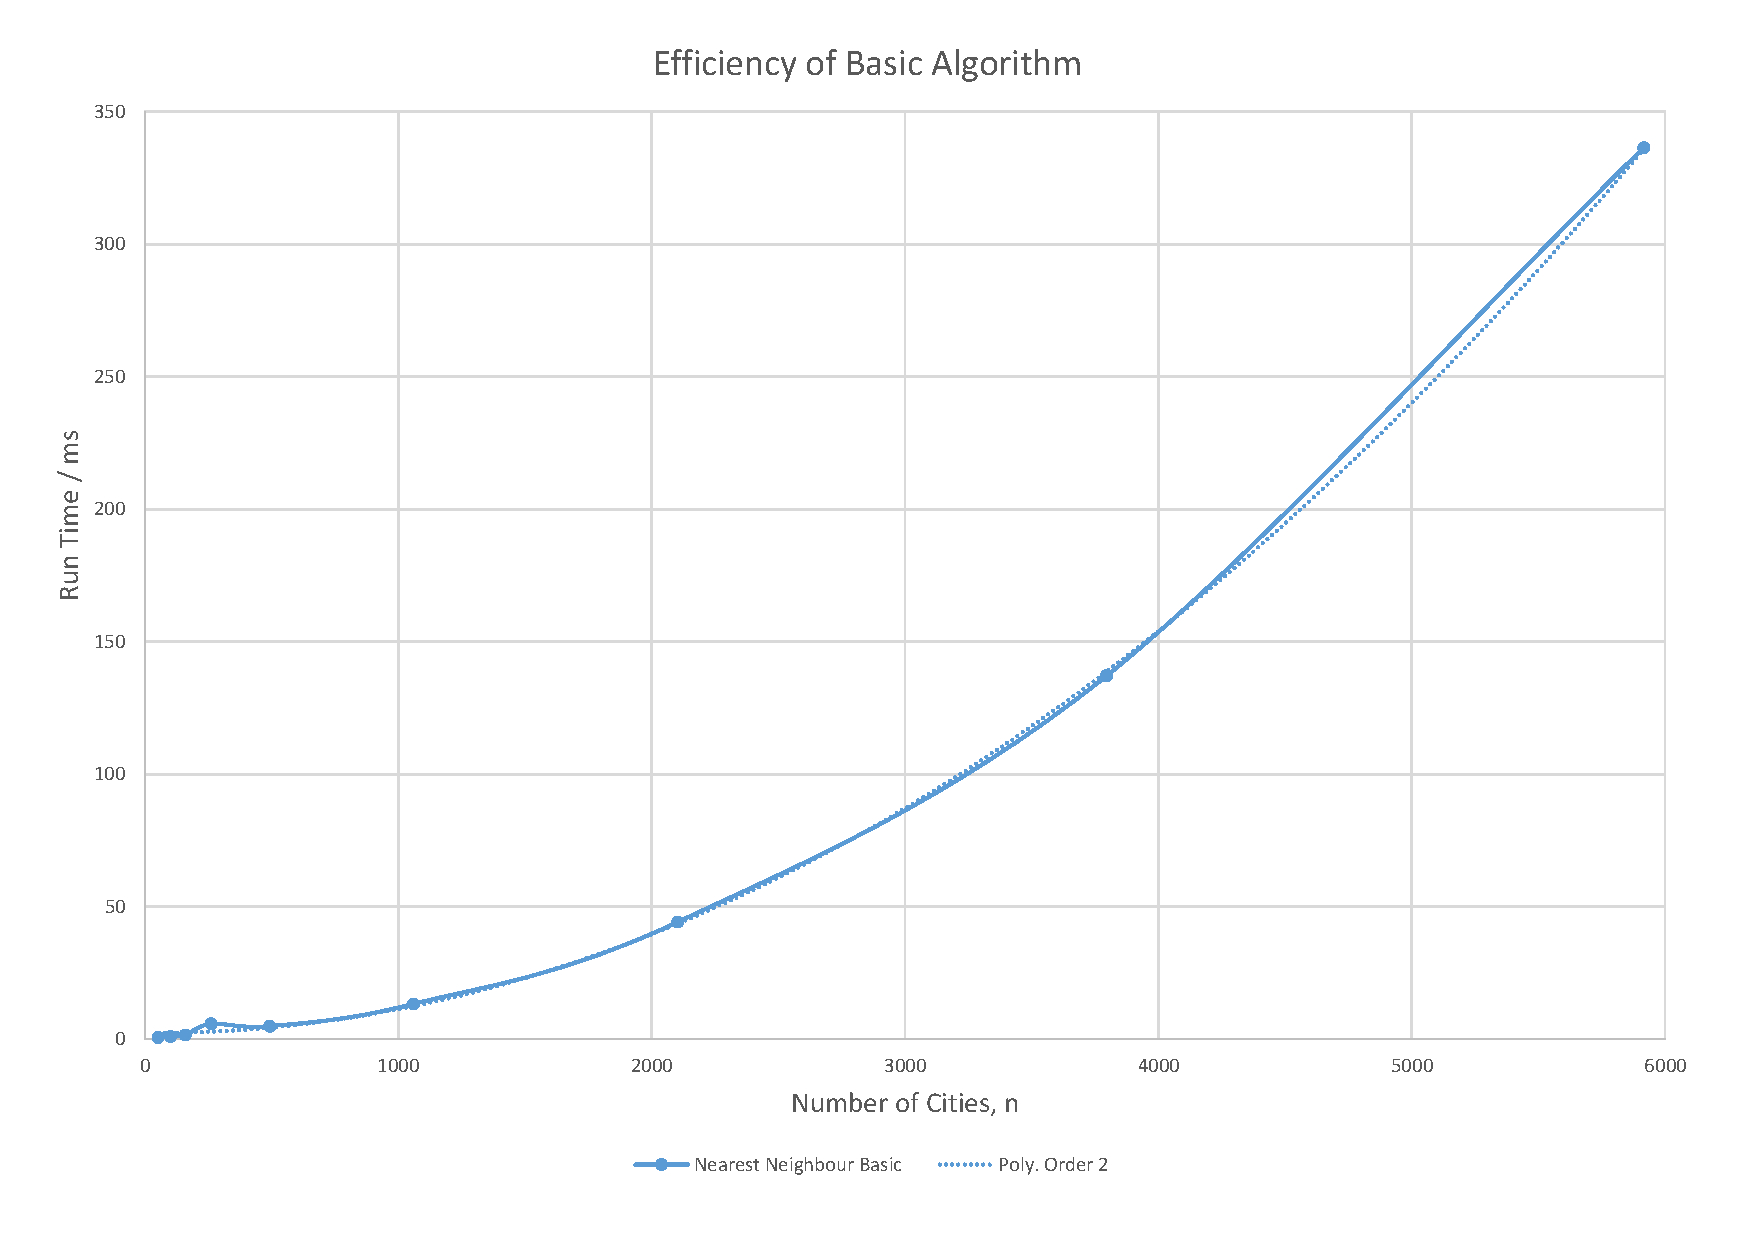
\includegraphics[width=\textwidth]{images/efficiency_basic.pdf}
	\caption{A graph showing the Nearest Neighbour Basic algorithm's average run time compared against the number of cities in each problem instance.}
	\label{fig2}
\end{figure*}

\section{Guidelines}
This section should be removed from your design report. Information provided here is to help you writing up your reports.

\begin{itemize}
\item Equations should be numbered and in the correct format, e.g., Equation \ref{eq:myequation} below:
\begin{equation} \label{eq:myequation}
 \sum_{j=1}^{z} j = \frac{z(z+1)}{2}
\end{equation}
\item Furthermore, if you include an equation, ensure you explain what each of the variables are (e.g., $F$ is force, $m$ is mass, and $a$ is the acceleration).
\item Don't using 'I' or 'Me'.
\item Each paragraph should be clear and focused, with multiple sentences that help make your point - avoid lots of single line paragraph sentence.
\item Make sure the citations are done using the correct formatting (i.e., .bib file and let LaTeX generate the references).
\item Every figure should have a caption, explaining what the picture is and what the reader should be looking at (i.e., what is important about the figure, what does it show)
\item A figure should also be referenced in the body of the main text (e.g., see Figure \ref{fig:teaser})
\item Equations should be numbered, and referenced in the text. Furthermore, ensure each of the variables in the equation are explained (i.e., don't use F=ma and not say what F, a, and m are)
\end{itemize}


\section{Conclusion and Future work}
The report should finish with a summary to give a brief overview of what the reader should remember most.  What was most important? The future work part only needs to be covered in your final report.


% \section*{Acknowledgements}


\bibliographystyle{acmsiggraph}
\bibliography{report}

\end{document}

